% A CONSORT-style flowchart of a randomized controlled trial
% using the PGF/TikZ package
% Author  : Morten Vejs Willert (July 2010)
% License : Creative Commons attribution license
\documentclass{article}
\usepackage[latin1]{inputenc}
\usepackage[margin=0.2in]{geometry}
\usepackage{tikz}
\usetikzlibrary{positioning,shapes,arrows,fit,calc}
\usepackage{caption}
\usepackage{amsmath}
\usepackage{verbatimbox}
\usepackage[framed]{matlab-prettifier}
\usepackage{filecontents}
\usepackage[scaled]{helvet}
\renewcommand\familydefault{\sfdefault} 
\usepackage[T1]{fontenc}
\usepackage[scaled]{beramono}
\usepackage{multicol}

\usepackage{xcolor}
\definecolor{oblue}{rgb}{0.4745,0.6,0.8}



% \tikzset{
%  font={\fontsize{10pt}{12}\selectfont}}

%  \vfill\null
%\columnbreak

% TODO rounded code block frames does not work with a background color
% (background color spills out of the rounded corner).
\lstset{
%frameround=tttt,
backgroundcolor=\color{oblue!10!white}
}

\begin{document}
\begin{center}

{\large\textbf{OpenSim Moco Cheat Sheet for Matlab Interface}}

  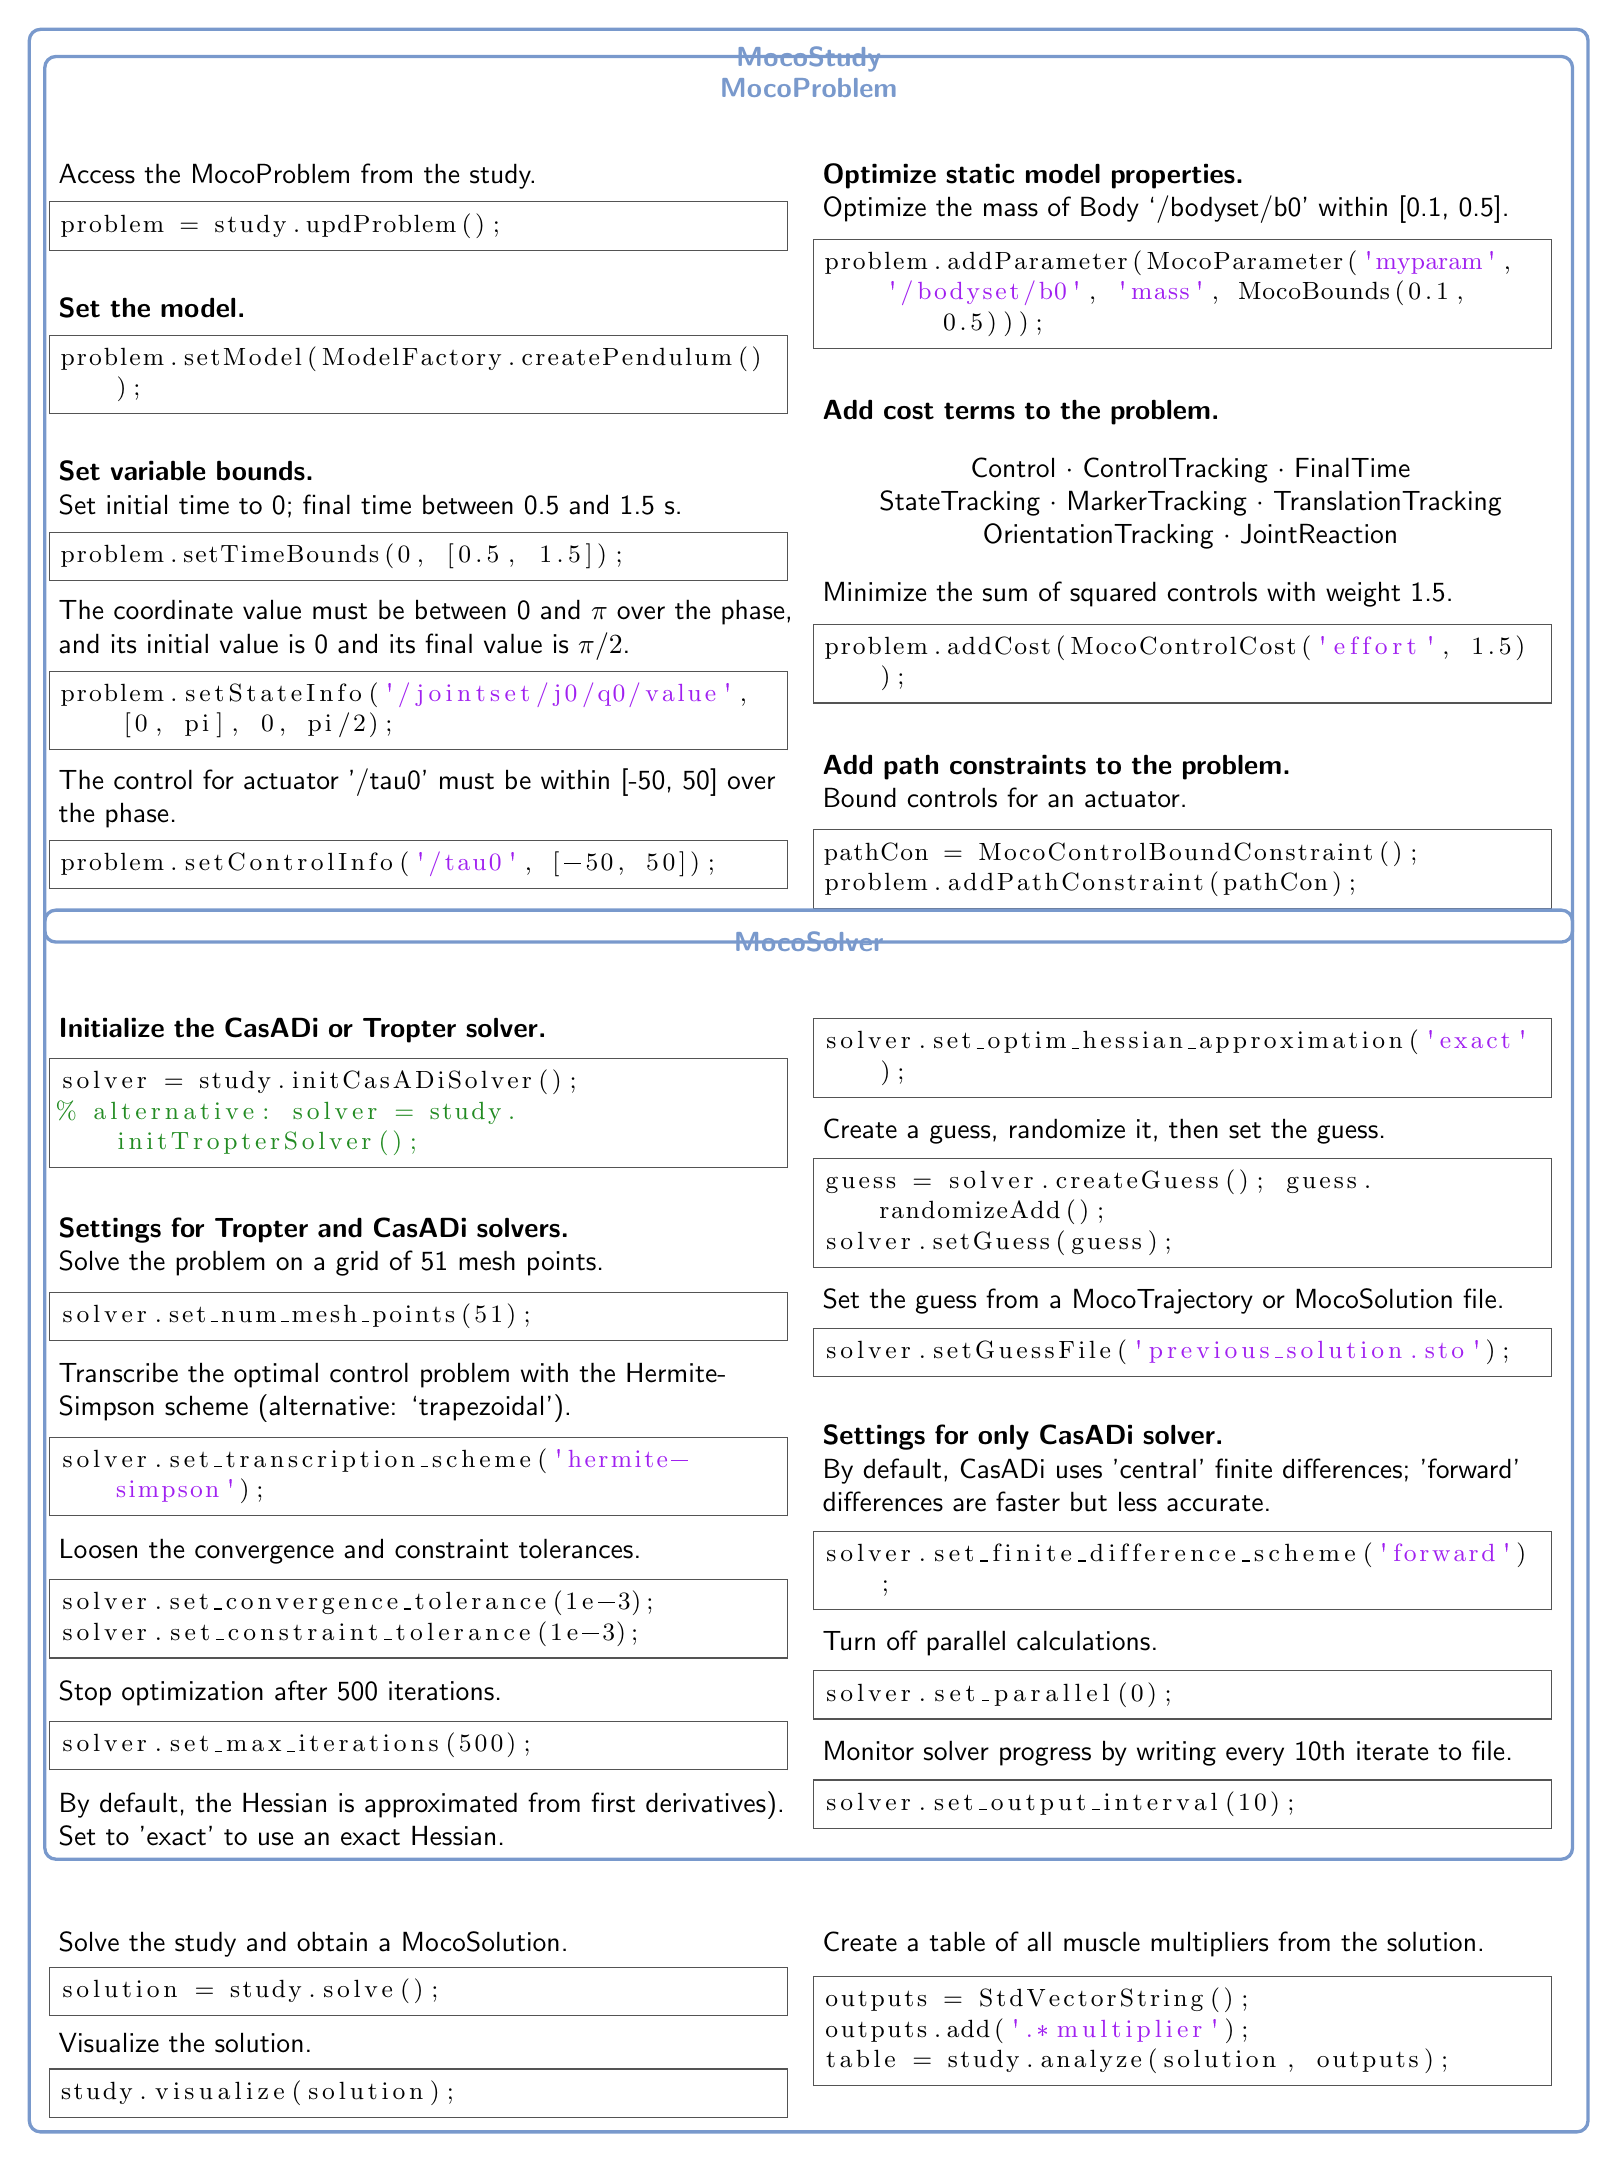
\begin{tikzpicture}[auto]
    
    
	\tikzstyle{object} = [draw=oblue, very thick,
    	rectangle, rounded corners, inner sep=5pt, inner ysep=5pt]
    
\node (studybody) [align=left, text width=7in] {
\vspace{-15pt}
\begin{center}\textbf{\textcolor{oblue}{MocoStudy}}\end{center}
};
    
    \node (problem) at ([shift={(270:5.3)}]studybody.south) [object, align=left, text width=7.5in] {
\vspace{-10pt}
\begin{center}\textbf{\textcolor{oblue}{MocoProblem}}\end{center}
\begin{multicols}{2}% 2-column layout
Access the MocoProblem from the study.
\begin{lstlisting}[style=Matlab-editor, basicstyle=\mlttfamily\small, linewidth=0.48\textwidth]
problem = study.updProblem();
\end{lstlisting}
\vspace{10pt}
\textbf{Set the model.}\\
\begin{lstlisting}[style=Matlab-editor, basicstyle=\mlttfamily\small, linewidth=0.48\textwidth]
problem.setModel(ModelFactory.createPendulum());
\end{lstlisting}
\vspace{10pt}
\textbf{Set variable bounds.}\\
Set initial time to 0; final time between 0.5 and 1.5 s.
\begin{lstlisting}[style=Matlab-editor, basicstyle=\mlttfamily\small, linewidth=0.48\textwidth]
problem.setTimeBounds(0, [0.5, 1.5]);
\end{lstlisting}
The coordinate value must be between 0 and $\pi$ over the phase, 
and its initial value is 0 and its final value is $\pi/2$.
\begin{lstlisting}[style=Matlab-editor, basicstyle=\mlttfamily\small, linewidth=0.48\textwidth]
problem.setStateInfo('/jointset/j0/q0/value', 
    [0, pi], 0, pi/2);
\end{lstlisting}
The control for actuator '/tau0' must be within [-50, 50] over the phase.
\begin{lstlisting}[style=Matlab-editor, basicstyle=\mlttfamily\small, linewidth=0.48\textwidth]
problem.setControlInfo('/tau0', [-50, 50]);
\end{lstlisting}
  \vfill\null
\columnbreak
\textbf{Optimize static model properties.}\\
Optimize the mass of Body `/bodyset/b0' within [0.1, 0.5].
\begin{lstlisting}[style=Matlab-editor, basicstyle=\mlttfamily\small, linewidth=0.48\textwidth]
problem.addParameter(MocoParameter('myparam',
    '/bodyset/b0', 'mass', MocoBounds(0.1, 0.5)));
\end{lstlisting}
\vspace{10pt}
\textbf{Add cost terms to the problem.}
\begin{center}
Control $\cdot $ ControlTracking $\cdot$ FinalTime \\
StateTracking $\cdot$ MarkerTracking $\cdot$ TranslationTracking \\
OrientationTracking $\cdot$ JointReaction
\end{center}
Minimize the sum of squared controls with weight 1.5.
\begin{lstlisting}[style=Matlab-editor, basicstyle=\mlttfamily\small, linewidth=0.48\textwidth]
problem.addCost(MocoControlCost('effort', 1.5));    
\end{lstlisting}
\vspace{10pt}
\textbf{Add path constraints to the problem.}\\
Bound controls for an actuator.
\begin{lstlisting}[style=Matlab-editor, basicstyle=\mlttfamily\small, linewidth=0.48\textwidth]
pathCon = MocoControlBoundConstraint();
problem.addPathConstraint(pathCon);
\end{lstlisting}
\end{multicols}
};
    
\node (solver) at ([shift={(270:5.6)}]problem.south) [object, align=left, text width=7.5in] {
\vspace{-10pt}
\begin{center}\textbf{\textcolor{oblue}{MocoSolver}}\end{center}
\begin{multicols}{2}% 2-column layout
\textbf{Initialize the CasADi or Tropter solver.}\\
\begin{lstlisting}[style=Matlab-editor, basicstyle=\mlttfamily\small, linewidth=0.48\textwidth]
solver = study.initCasADiSolver();
% alternative: solver = study.initTropterSolver();
\end{lstlisting}
\vspace{10pt}
\textbf{Settings for Tropter and CasADi solvers.}\\
Solve the problem on a grid of 51 mesh points.
\begin{lstlisting}[style=Matlab-editor, basicstyle=\mlttfamily\small, linewidth=0.48\textwidth]
solver.set_num_mesh_points(51);
\end{lstlisting}
Transcribe the optimal control problem with the Hermite-Simpson scheme (alternative: `trapezoidal').
\begin{lstlisting}[style=Matlab-editor, basicstyle=\mlttfamily\small, linewidth=0.48\textwidth]
solver.set_transcription_scheme('hermite-simpson');
\end{lstlisting}
Loosen the convergence and constraint tolerances.
\begin{lstlisting}[style=Matlab-editor, basicstyle=\mlttfamily\small, linewidth=0.48\textwidth]
solver.set_convergence_tolerance(1e-3);
solver.set_constraint_tolerance(1e-3);
\end{lstlisting}
Stop optimization after 500 iterations.
\begin{lstlisting}[style=Matlab-editor, basicstyle=\mlttfamily\small, linewidth=0.48\textwidth]
solver.set_max_iterations(500);
\end{lstlisting}
By default, the Hessian is approximated from first derivatives). Set to 'exact' to use an exact Hessian.
\begin{lstlisting}[style=Matlab-editor, basicstyle=\mlttfamily\small, linewidth=0.48\textwidth]
solver.set_optim_hessian_approximation('exact');
\end{lstlisting}
Create a guess, randomize it, then set the guess.
\begin{lstlisting}[style=Matlab-editor, basicstyle=\mlttfamily\small, linewidth=0.48\textwidth]
guess = solver.createGuess(); guess.randomizeAdd();
solver.setGuess(guess);
\end{lstlisting}
Set the guess from a MocoTrajectory or MocoSolution file.
\begin{lstlisting}[style=Matlab-editor, basicstyle=\mlttfamily\small, linewidth=0.48\textwidth]
solver.setGuessFile('previous_solution.sto');
\end{lstlisting}

\vspace{10pt}
\textbf{Settings for only CasADi solver.}\\
By default, CasADi uses 'central' finite differences; 'forward' differences are faster but less accurate.
\begin{lstlisting}[style=Matlab-editor, basicstyle=\mlttfamily\small, linewidth=0.48\textwidth]
solver.set_finite_difference_scheme('forward');
\end{lstlisting}
Turn off parallel calculations.
\begin{lstlisting}[style=Matlab-editor, basicstyle=\mlttfamily\small, linewidth=0.48\textwidth]
solver.set_parallel(0);
\end{lstlisting}
Monitor solver progress by writing every 10th iterate to file.
\begin{lstlisting}[style=Matlab-editor, basicstyle=\mlttfamily\small, linewidth=0.48\textwidth]
solver.set_output_interval(10);
\end{lstlisting}
\end{multicols}
};

\node (studypost) at ([shift={(270:1.6)}]solver.south) [align=left, text width=7.5in] {
\begin{multicols}{2}% 2-column layout
    
Solve the study and obtain a MocoSolution.
\begin{lstlisting}[style=Matlab-editor, basicstyle=\mlttfamily\small, linewidth=0.48\textwidth]
solution = study.solve();
\end{lstlisting}
Visualize the solution.
\begin{lstlisting}[style=Matlab-editor, basicstyle=\mlttfamily\small, linewidth=0.48\textwidth]
study.visualize(solution);
\end{lstlisting}
Create a table of all muscle multipliers from the solution.
\begin{lstlisting}[style=Matlab-editor, basicstyle=\mlttfamily\small, linewidth=0.48\textwidth]
outputs = StdVectorString();
outputs.add('.*multiplier');
table = study.analyze(solution, outputs);
\end{lstlisting}
\end{multicols}
};
    
    
    \node (study) [object, fit={(studybody) (problem) (solver) (studypost)}] {};
%      	\begin{equation*}
%      	    \begin{alignat*}{2}
%        \mbox{minimize}
%         \quad & \sum_j w_{E,j} \left(J_{E,j}(t_0, t_f, y_0, y_f, x_{0}, x_{f}, \lambda_0, \lambda_f, p)
%         + \int_{t_0}^{t_f} J_{I,j}(t, y, x, \lambda, p)~dt\right) &&  \\
%        \mbox{subject to}
%         \quad & \dot{q} = u \\
%         & M(q, p)\dot{u} + G(q, p)^T \lambda = f_{\textrm{app}}(t, y, x, p) - f_{\textrm{bias}}(q, u, p) \\
%         & \dot{z}(t) = f_{\textrm{aux}}(t, y, x, \lambda, p) \\
%         & 0 = \phi(q, p) \\
%         & 0 = \nu(q, u, p) \\
%         & 0 = \alpha(q, u, \dot{u}, p) \\
%         & g_{L} \leq g(t, y, x, \lambda, p) \leq g_{U} \\
%         & y_{0,L} \leq y_0 \leq y_{0,U} \\
%         & x_{0,L} \leq x_0 \leq x_{0,U} \\
%         & y_{f,L} \leq y_f \leq y_{f,U} \\
%         & x_{f,L} \leq x_f \leq x_{f,U} \\
%         \mbox{with respect to} \quad
%         & y \in [y_{L}, y_{U}] \\
%         & x \in [x_{L}, x_{U}] \\
%         & p \in [p_{L}, p_{U}] \\
%         & t_0 \in [t_{0,L}, t_{0,U}] \\
%         & t_f \in [t_{f,L}, t_{f,U}]
%    \end{alignat*}
%    \end{equation*}
  \end{tikzpicture}
\end{center}
\newpage



\end{document}

% TODO
% add equations to the back side
% add MocoTrajectory interface
% add generic functions in MocoStudy.
% solve()
% visualize()
% analyze()
% add Utilities

%    block_center/.style ={
%    	rectangle, rounded corners,
%    	draw=black, very thick,
%      	text width=8em, text centered,
%      	minimum height=4em,
%      	inner sep=10pt,
%      	inner ysep=10pt,
%      	% minimum width=50em,
%      },
%    block_left/.style ={
%    	rectangle, rounded corners,
%    	draw=black, very thick,
%      	text width=8em,
%      	minimum height=4em,
%      	inner sep=10pt,
%      	inner ysep=10pt,
%      	minimum width=50em
%      	},
%    block_noborder/.style ={rectangle, draw=none, thick, fill=none,
%      text width=18em, text centered, minimum height=1em},
%    block_assign/.style ={rectangle, draw=black, thick, fill=white,
%      text width=18em, text ragged, minimum height=3em, inner sep=6pt},
%    block_lost/.style ={rectangle, draw=black, thick, fill=white,
%      text width=16em, text ragged, minimum height=3em, inner sep=6pt},
%      line/.style ={draw, thick, -latex', shorten >=0pt}]
%
%
